\chapter{Implementacja}
\label{cha:implementacja}


%---------------------------------------------------------------------------

\section{Implementacja modelu HMR}
\label{sec:implementacjaModeluHmr}

\subsection{Konstruowanie modelu wnioskującego}

Plugin \textit{HowAreYou} został stworzony w ten sposób, że wszystkie reguły wnioskujące silnika \textit{HeaRTDroid} mieszczą się poza kodem źródłowym aplikacji. W strukturze projektu \textit{Android Studio} pliki dodatkowe umieszcza się zazwyczaj w katalogu \textit{assets} - tak jest rownież z plikiem \textit{model.hmr}, który zawiera szczegółowy opis reguł w języku zrozumiałym dla silnika wnioskującego.

Do tworzenia pliku \textit{model.hmr} wykorzystana została aplikacja webowa \textit{HeaKatE Web Editor} (w skrócie \textit{HWEd}). \textit{HWEd} jest edytorem online (stworzonym z wykorzystaniem środowiska \textit{node.js}) służącym do tworzenia i edytowania modeli, które później wykorzystywane są przez silnik wnioskujący \textit{HeaRTDroid} \cite{heartdroid}. Zawarty w nim parser przetwarza reguły \textit{XTT2} na czytelne dla użytkownika zestawy połączonych ze sobą tabel, a następnie po wybraniu opcji \textit{Export} przekształca tablice w plik HMR z regułami \textit{XTT2} \cite{heartdroid}.

Samo \textit{XTT2} jest formalizmem reprezentacji wiedzy stworzonym z myślą o regułach. Służy algebraicznej i logicznej specyfikacji reguł pozwalając na zwięzły, przejrzysty i efektywny sposób wizualnej reprezentacji wiedzy. W odróżnieniu od tradycyjnych systemów pozwala wykorzystanie "płaskiego" (jednoopoziomowego) zestawu reguł. Wprowadza tablice, wykorzystywane do reprezentowania zestawów regół mających podobrą strukturę, oraz połączenia między tablicami. Struktura zestawów tabel przypomina drzewa decyzyjne \cite{AiWikiHekate}.

Podczas opracowywania modelu wykorzystane zostało również narzędzie \textit{HeaRTDroid Query Notation} (w skrócie \textit{HaQuNa}). \textit{HaQuNa} jest prostym językiem, który może być wykorzystywane w interaktywnej powłoce. Zestaw poleceń linii komend umożliwia wczytywanie, modyfikację oraz uruchamianie modeli HMR\cite{heartdroid}. Przy implementacji \textit{HowAreYou} \textit{HaQuNa} była wykorzystywana do weryfikacji poprawności tworzonego modelu.

Należy jeszcze podkreślić, że plik modelu architektonicznie oddzielony został od implementacji aplikacji. Dzięki zastosowaniu tego rozwiązania, plugin \textit{HowAreYou} nie musi być powiązany z obecnie zaimplementowanym domyślnym modelem. Ekspert domenowy, który nie musi być nawet osobą techniczną, może bez trudu z wykorzystaniem edytora online stworzyć nowy zestaw reguł \textit{XTT2} i zastąpić w strukturze projektu plik \textit{model.hmr}.

\subsection{Zaawansowany model wnioskujący}

\subsubsection{Realizacja zaawansowanego modelu wnioskującego}

Celem realizacji zaawansowanego modelu wnioskującego było opracowanie modelu, z pomocą którego zostaną wybrane jak najlepszy moment i sposób na zapytanie użytkownika o jego samopoczucie. Możliwe jest zapytanie niejawne poprzez wykonanie i przetworzenie fotografii lub zapytanie jawne - o kolor lub bezpośrednio o emocje.

W procesie wnioskowania brane są pod uwagę czynniki takie jak czas jaki upłynął od ostatniego zapytania, korzystanie z nawigacji samochodowej, wykonywanie połączenia telefonicznego, oglądanie filmów, czy wykonywanie ruchu. Uwzględniane są też wyniki analizy fotografii oraz wiedza, czy w danej chwili użytkownik korzysta z ekranu telefonu.

Poniższe obrazy przedstawiają widok modelu HMR w edytorze \textit{HWEd}. Model został skonstruowany jako zestaw tabel, które zależąc od informacji z aplikacji oraz od siebie nawzajem realizują reguły decyzyjne. Decyzja z jednej tabeli ma bezpośreni wpływ na działanie kolejnej. Ostatecznie zgodnie z wynikiem z ostatniej tabeli \textit{howareyouAction} plugin \textit{HowAreYou} podejmuje określoną akcję.

\begin{figure}[H]
	\centering
	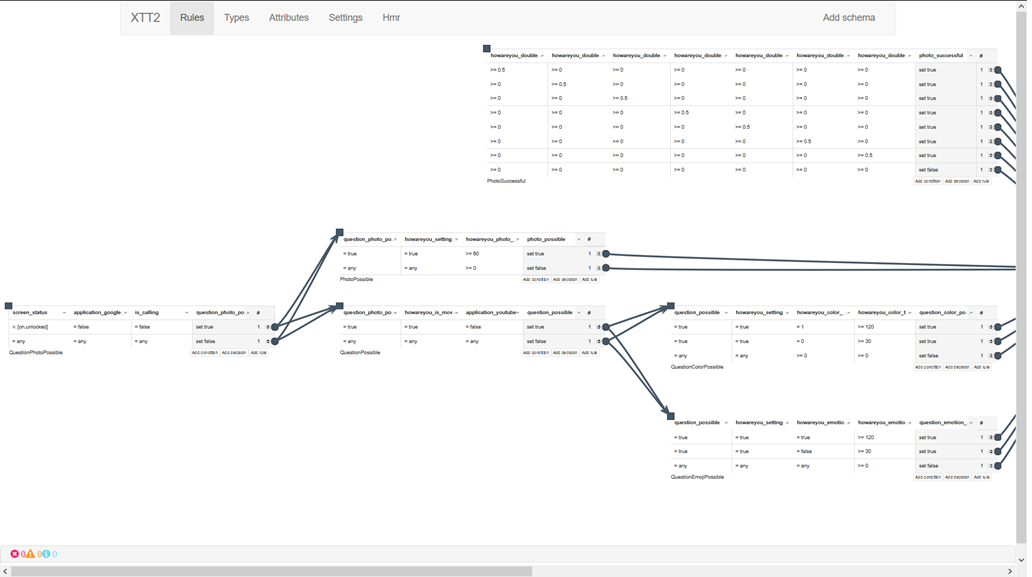
\includegraphics[scale=0.8]{rozdzial4/HMR_advancedModelPart1.png}
	\caption{Zaawansowany model wnioskujący: część 1.}
\end{figure}

\begin{figure}[H]
\centering
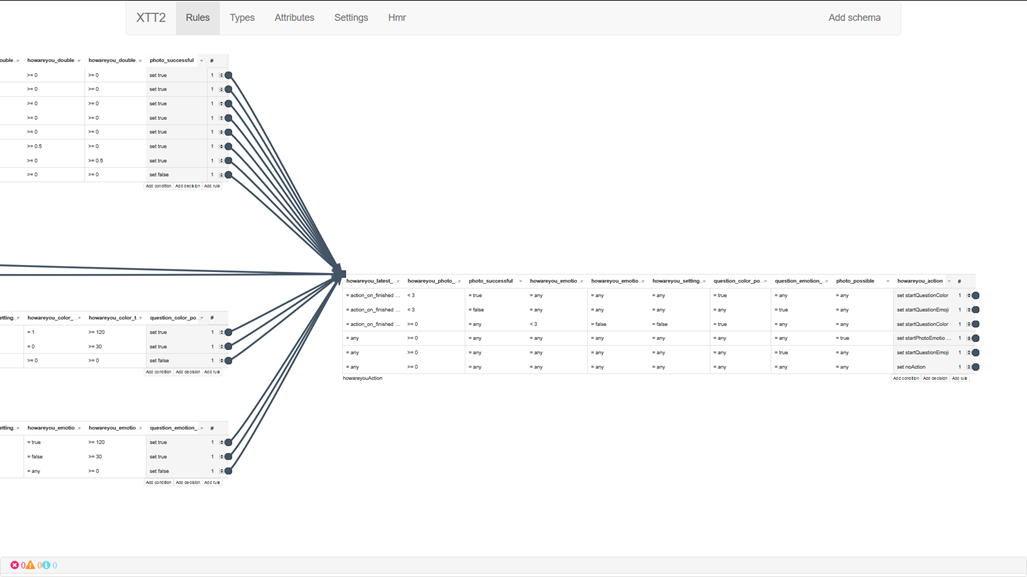
\includegraphics[scale=0.8]{rozdzial4/HMR_advancedModelPart2.png}
\caption{Zaawansowany model wnioskujący: część 2.}
\end{figure}

W kolejnej części rozdziału omawiane zostają krok po kroku zasady działania poszczególnych tabel powyższego modelu.


\subsubsection{Tabela QuestionPhotoPossible}

\begin{enumerate}
	\item Tabela zwraca prawdę, jeżeli spełnione są wspólne warunki konieczne do zapytania użytkownika lub wykonania zdjęcia.
	\item Żeby uruchomić pytanie lub zrobić zdjęcie ekran telefonu musi być aktywny, telefon nie może prowadzić nawigacji, ani wykonywać połączenia.
\end{enumerate}

\begin{figure}[H]
	\centering
	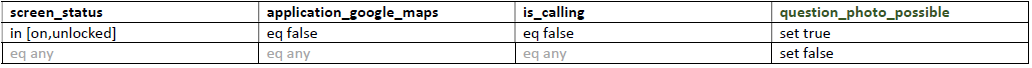
\includegraphics[scale=0.8]{rozdzial4/HMR_QuestionPhotoPossible.png}
	\caption{Zaawansowany model wnioskujący: tabela QuestionPhotoPossible.}
\end{figure}


\subsubsection{Tabela PhotoPossible}

\begin{enumerate}
\item Tabela zwraca prawdę, jeżeli spełnione są warunki konieczne do wykonania zdjęcia.
\item Żeby zrobić zdjęcie telefon musi spełniać warunki konieczne wspólne dla zdjęcia i pytania. Dodatkowo opcja wykonywania zdjęć musi być uruchomiona i czas, jaki upłynął od ostatniego zdjęcia, musi być większy lub równy 60 minut.

\end{enumerate}

\begin{figure}[H]
\centering
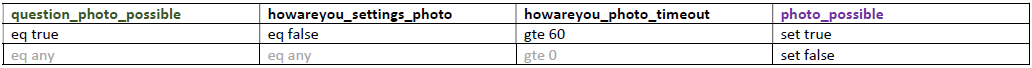
\includegraphics[scale=0.8]{rozdzial4/HMR_PhotoPossible.png}
\caption{Zaawansowany model wnioskujący: tabela PhotoPossible.}
\end{figure}


\subsubsection{Tabela QuestionPossible}

\begin{enumerate}
\item Tabela zwraca prawdę, jeżeli spełnione są warunki konieczne do zapytania użytkownika.
\item Żeby uruchomić pytanie telefon musi spełniać warunki konieczne wspólne dla zdjęcia i pytania. Dodatkowo musi znajdować się w ruchu (jeżeli jest w bezruchu, najprawdopodobniej jest odłożony) i nie może być uruchomiona aplikacja do oglądania filmów. 
\end{enumerate}

\begin{figure}[H]
\centering
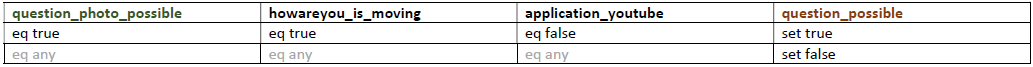
\includegraphics[scale=0.8]{rozdzial4/HMR_QuestionPossible.png}
\caption{Zaawansowany model wnioskujący: tabela QuestionPossible.}
\end{figure}


\subsubsection{Tabela QuestionColorPossible}

\begin{enumerate}
\item Tabela zwraca prawdę, jeżeli spełnione są warunki konieczne do zapytania użytkownika o kolor.
\item Żeby uruchomić pytanie o kolor telefon musi spełniać warunki konieczne do zadania pytania. Dodatkowo ustawienia pluginu muszą pozwalać zapytać o kolor. Jeżeli ostatnie pytanie o kolor było odrzucone, kolejne pytanie może być zadane po 120 minutach. Jeżeli nie było odrzucone – po 30 minutach.


\end{enumerate}

\begin{figure}[H]
\centering
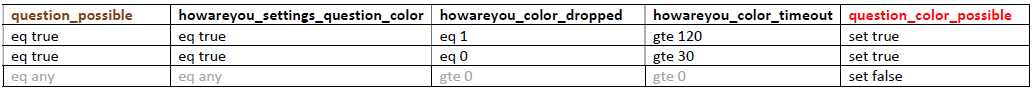
\includegraphics[scale=0.8]{rozdzial4/HMR_QuestionColorPossible.png}
\caption{Zaawansowany model wnioskujący: tabela QuestionColorPossible.}
\end{figure}


\subsubsection{Tabela QuestionEmojiPossible}

\begin{enumerate}
\item Tabela zwraca prawdę, jeżeli spełnione są warunki konieczne do zapytania użytkownika o emocje.
\item Żeby uruchomić pytanie o emocje telefon musi spełniać warunki konieczne do zadania pytania. Dodatkowo ustawienia pluginu muszą pozwalać zapytać o emocje. Jeżeli ostatnie pytanie o emocje było odrzucone, kolejne pytanie może być zadane po 120 minutach. Jeżeli nie było odrzucone – po 30 minutach.


\end{enumerate}

\begin{figure}[H]
\centering
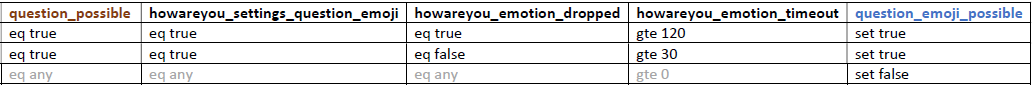
\includegraphics[scale=0.8]{rozdzial4/HMR_QuestionEmojiPossible.png}
\caption{Zaawansowany model wnioskujący: tabela QuestionEmojiPossible.}
\end{figure}


\subsubsection{Tabela PhotoSuccessful}

\begin{enumerate}
\item Tabela zwraca prawdę, jeżeli najnowsze zdjęcie w bazie danych uznaje się za udane.
\item Żeby uznać zdjęcie za udane wystarczy, że wartość prawdopodobieństwa jednej z wykrytych emocji (za wyjątkiem emocji neutral) jest większa niż próg (który obecnie wynosi 50%).
\end{enumerate}

\begin{figure}[H]
\centering
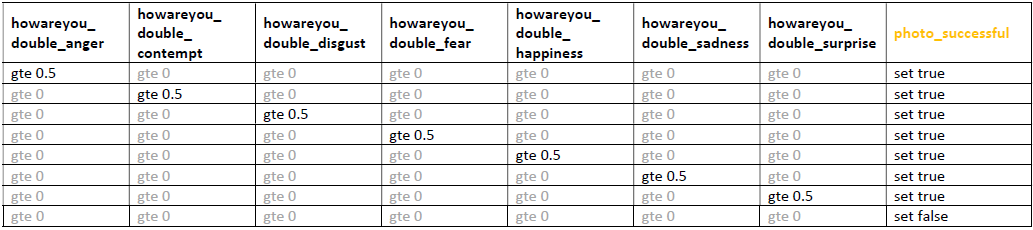
\includegraphics[scale=0.8]{rozdzial4/HMR_PhotoSuccessful.png}
\caption{Zaawansowany model wnioskujący: tabela PhotoSuccessful.}
\end{figure}


\subsubsection{Tabela howareyouAction}

Tabela zwraca prawdę, jeżeli najnowsze zdjęcie w bazie danych uznaje się za udane. 
\begin{enumerate}
\item Jeżeli ostatnią akcją jaką plugin wykonał było zdjęcie i to zdjęcie było niedawno (mniej niż 3 minuty temu) i to zdjęcie było udane, to telefon zapyta o kolor, jeżeli spełnione są warunki do zapytania o kolor.
\item Jeżeli ostatnią akcją jaką plugin wykonał było zdjęcie i to zdjęcie było niedawno (mniej niż 3 minuty temu), ale nie było udane, to telefon zapyta o emocje, jeżeli spełnione są warunki do zapytania o emocje.
\item Jeżeli ostatnią akcją jaką plugin wykonał było pytanie o emocje i to pytanie o emocje było niedawno (mniej niż 3 minuty temu) i użytkownik odpowiedział na to pytanie, to telefon zapyta o kolor, jeżeli spełnione są warunki do zapytania o kolor. Ta reguła (de facto dwa pytania jedno po drugim) wykona się tylko wtedy, gdy użytkownik w ustawieniach wyłączył wykonywanie zdjęć. 
\item Jeżeli jest możliwe zrobienie zdjęcia, to telefon wykona zdjęcie. 
\item Jeżeli nie jest możliwe zrobienie zdjęcia, to telefon zapyta o emocje, jeżeli spełnione są warunki do zapytania o emocje.
\item Jeżeli żadna z akcji nie jest możliwa, telefon nie wykona akcji.
\end{enumerate}

\begin{figure}[H]
\centering
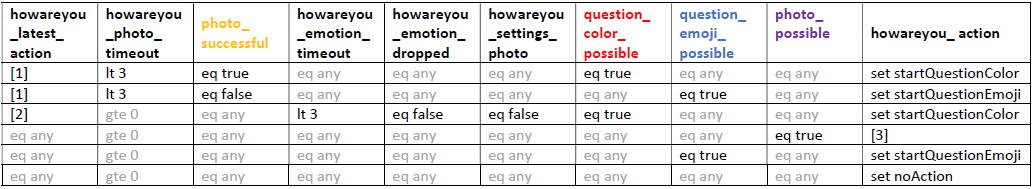
\includegraphics[scale=0.8]{rozdzial4/HMR_howareyouAction.png}
\caption{Zaawansowany model wnioskujący: tabela howareyouAction.}
\end{figure}


\subsubsection{Obserwowanie reguł wnioskujących}

Działanie systemu wnioskującego wykorzystującego zaawansowany model wnioskujący można obserwować na bieżąco z wykorzystaniem trybu debugowego. Po wybraniu opcji \textit{Otwórz log z ostatniego wnioskowania} w ustawieniach pluginu \textit{HowAreYou}, oczom użytkownika ukaże się okno ze szczegółowym opisem elementów wnioskowania: tabel, reguł i decyzji, jakie zostały podjęte.

\begin{figure}[H]
	\centering
	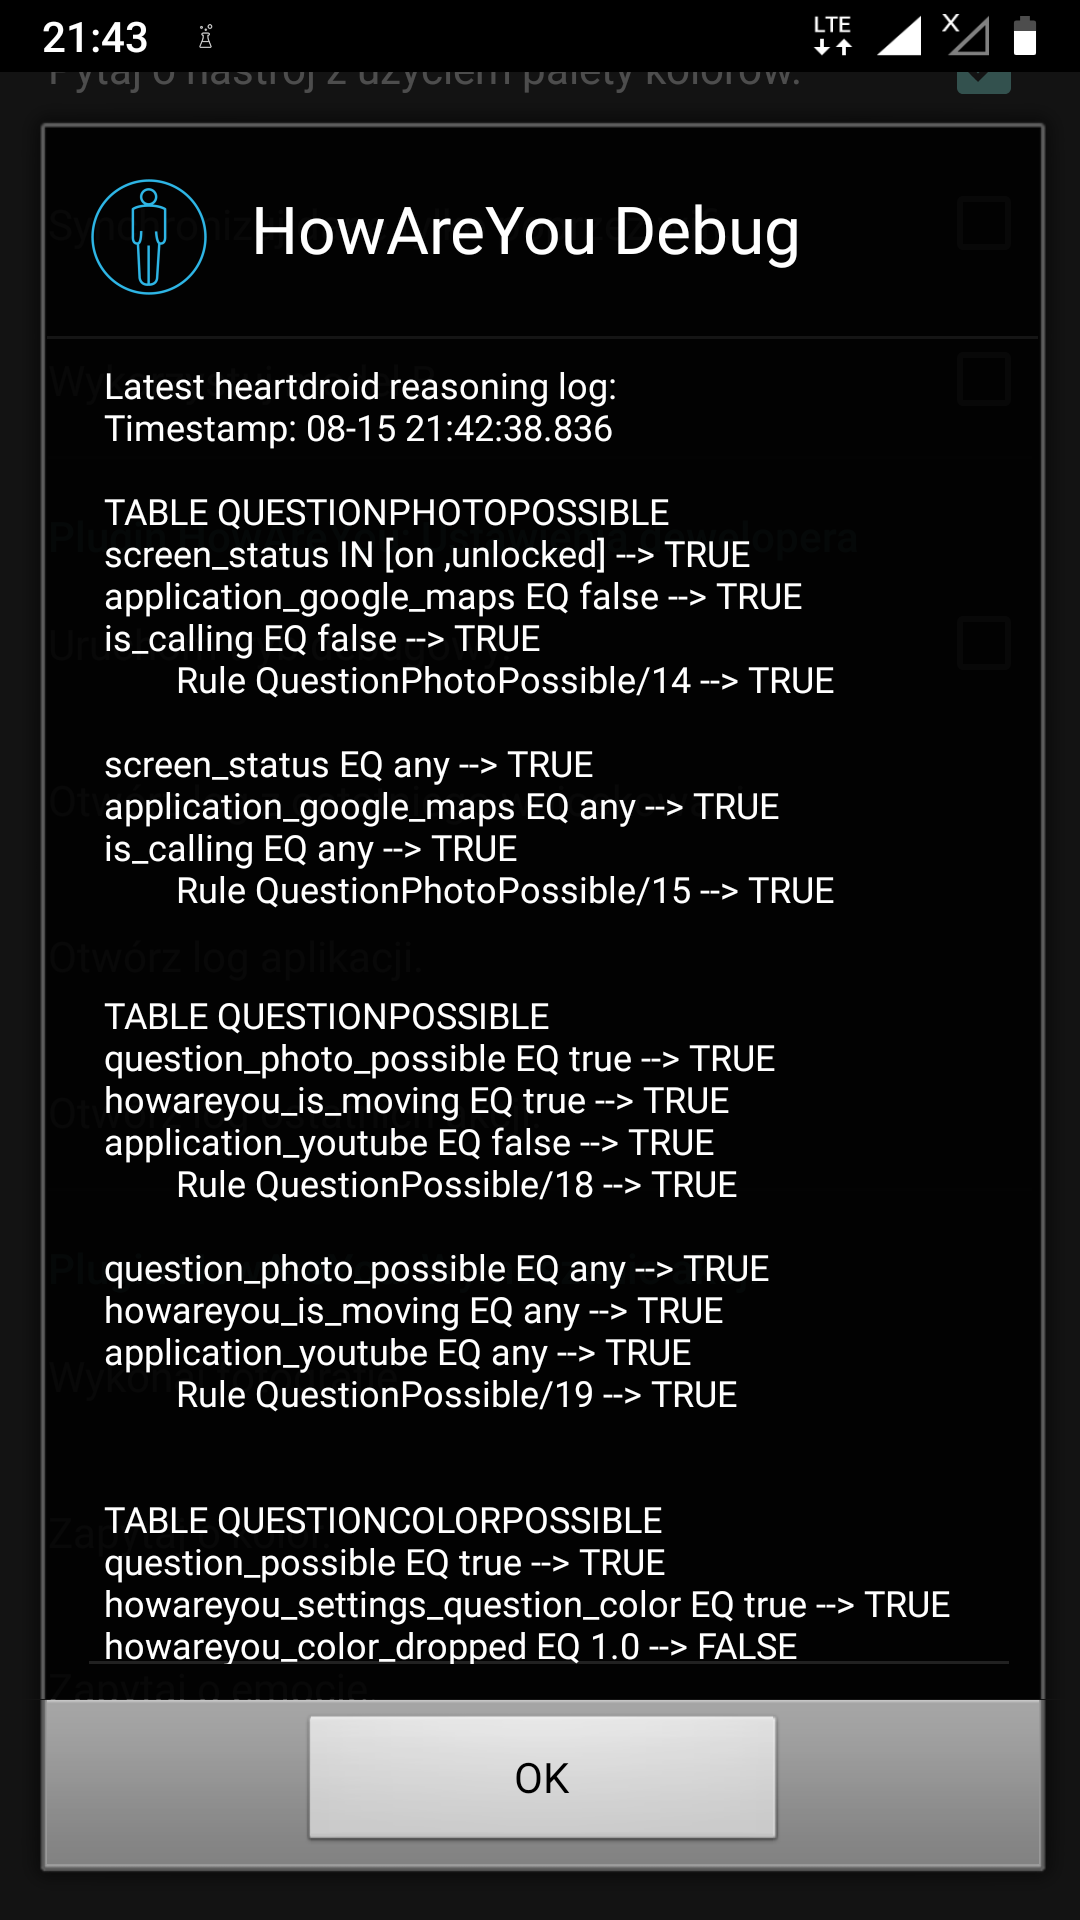
\includegraphics[scale=0.15]{rozdzial4/HMR_screenshots_A.png}
	\caption{Zaawansowany model wnioskujący: tabela howareyouAction.}
\end{figure}



\subsection{Uproszczony model wnioskujący}


\subsubsection{Realizacja uproszczonego modelu wnioskującego}

W celach badawczych został stworzony również model uproszczony. Dzięki niemu osoba przeprowadzająca badanie jest w stanie porównać, jaki wpływ na odbieranie przez uczestnika uciążliwości badania ma złożoność samego modelu. Model prosty został stworzony w kontraście do pierwszego modelu. Sam model wykorzystuje tylko 2 czynniki: wiedzę czy ekran jest urządzenia włączony oraz czas od ostatniego zapytania. Model  symuluje prosty i toporny system odpytywania użytkownika. 

Zdecydowaną zaletą \textit{HowAreYou} jest fakt, iż w celach porównawczych nie było niezbędne tworzenie dodatkowej aplikacji, która odpytywałaby użytkownika w sposób uproszczony, ani nawet modyfikacja kodu źródłowego aplikacji. Jedyną potrzebną czynnością była zmiana samego modelu HMR. Model uproszczony można aktywować w ustawieniach aplikacji. Można również zainstalować plugin \textit{HowAreYou} bezpośrednio z modelem uproszczonym. Podczas pobierania pliku instalatora należy wybrać wersję B (patrz: dodatek A).


\subsubsection{Tabela howareyouAction}

Tabela zwraca prawdę, jeżeli najnowsze zdjęcie w bazie danych uznaje się za udane. 
\begin{enumerate}
	\item Jeżeli ekran urządzenia jest aktywny i od ostatniego zapytania minęło co najmniej 60 minut, aplikacja zapyta użytkownika o emocje.
	\item Jeżeli któryś z powyższych warunków nie jest spełniony, telefon nie wykona żanej akcji.
\end{enumerate}

\begin{figure}[H]
	\centering
	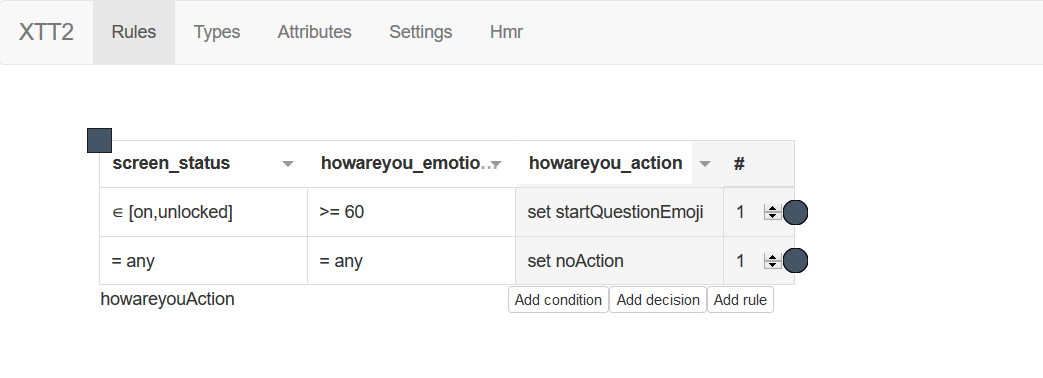
\includegraphics[scale=0.8]{rozdzial4/HMR_basic.png}
	\caption{Uproszczony model wnioskujący: tabela howareyouAction.}
\end{figure}

\subsubsection{Obserwowanie reguł wnioskujących}

Podobnie jak w przypadku zaawansowanego modelu, działanie systemu wnioskującego wykorzystującego uproszczony model można obserwować na bieżąco z wykorzystaniem trybu debugowego. Tutaj jednak log z wnioskowania jest znacznie krótszy - do tego stopnia, że obejmuje tylko jedną tabelę i tylko dwie reguły.

\begin{figure}[H]
	\centering
	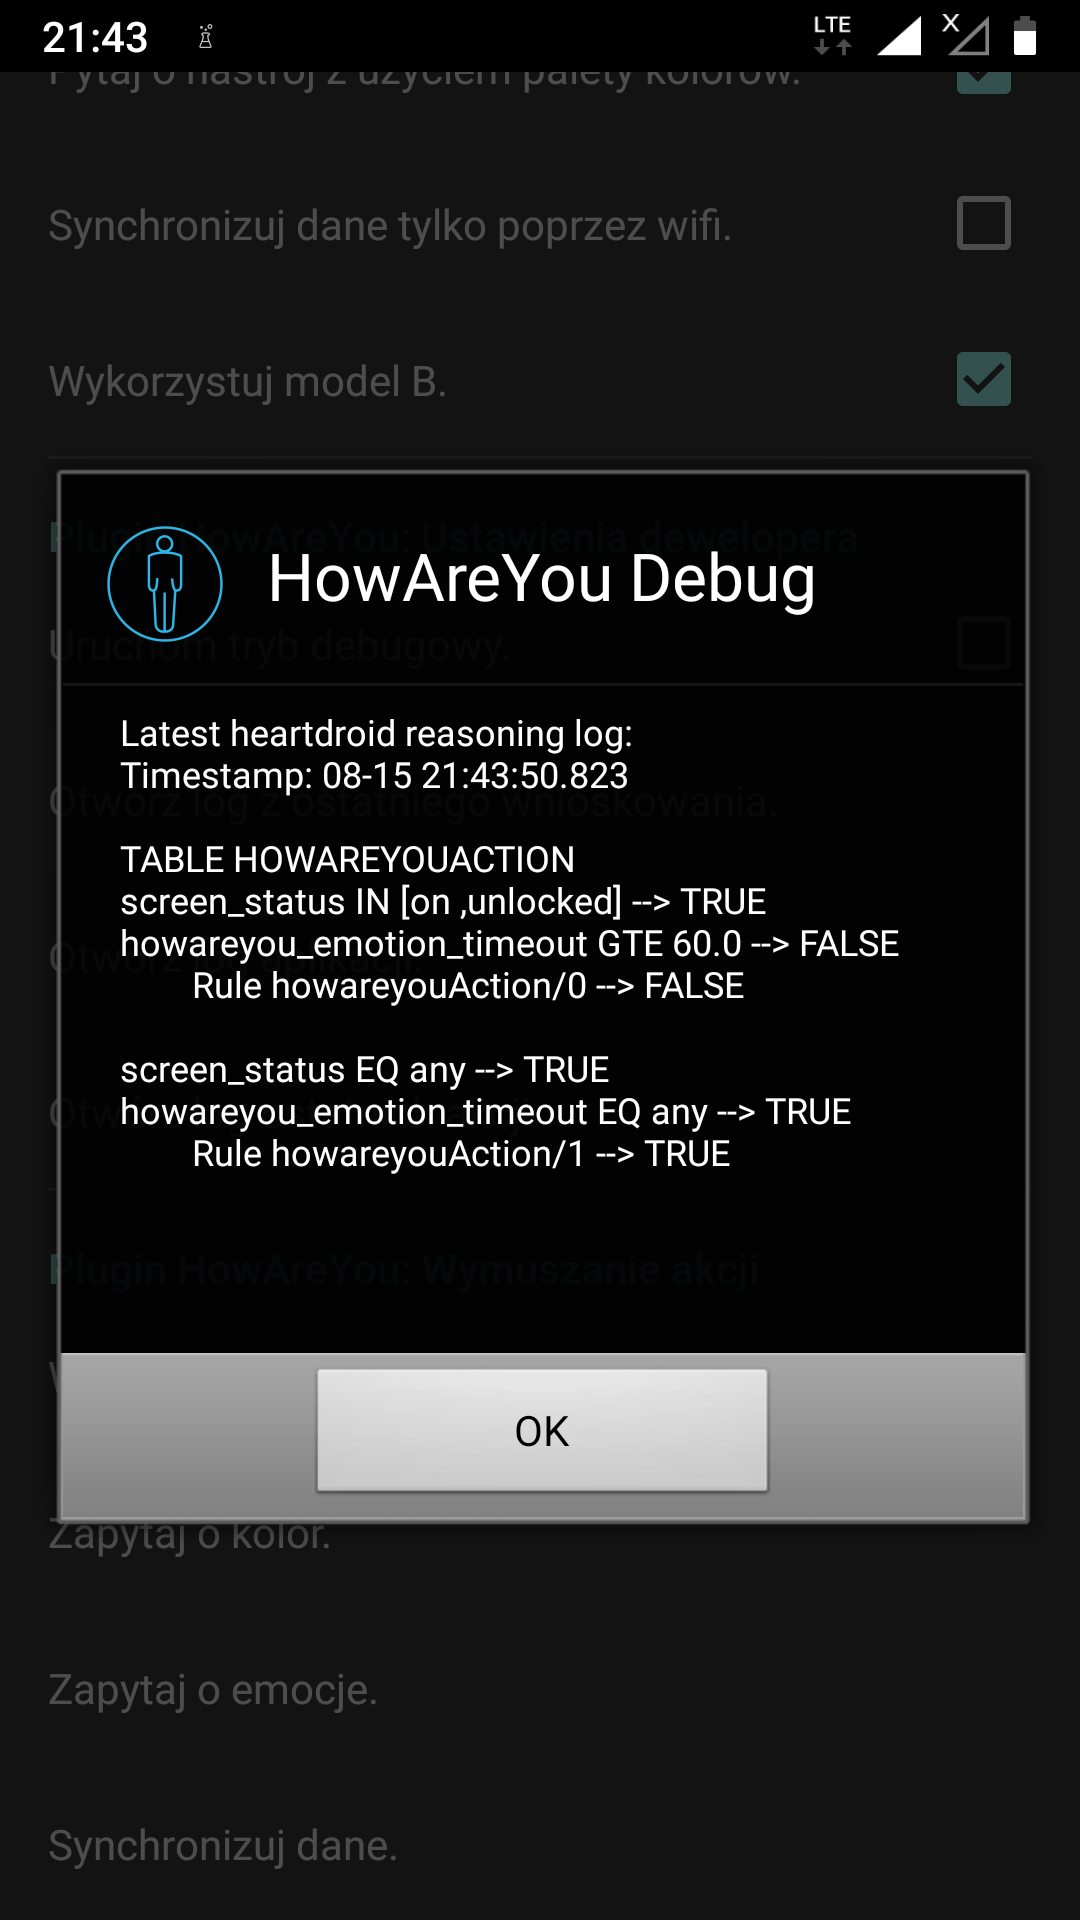
\includegraphics[scale=0.15]{rozdzial4/HMR_screenshots_B.png}
	\caption{Zaawansowany model wnioskujący: tabela howareyouAction.}
\end{figure}